
\begin{frame} {Semiconductor Devices in 3D: FinFET} 
  
 \begin{center} 
   {\footnotesize Intel Trigate transistors} \\
   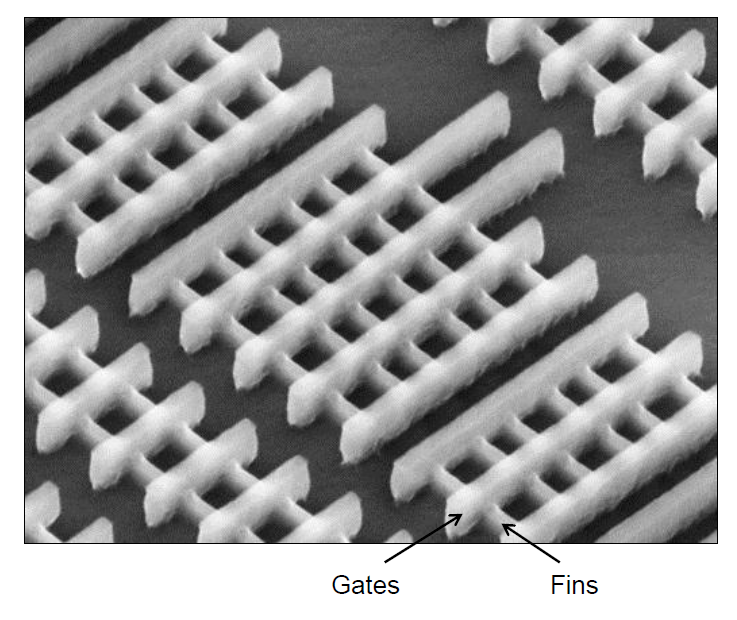
\includegraphics[width=0.7\textwidth]{intel-trigate}
 \end{center} 
{\tiny http://download.intel.com/newsroom/kits/22nm/gallery/images/Intel-22nm\_Transistor\_2.jpg} \\[.6em]
 
\end{frame} 


\begin{frame} {Semiconductor Devices in 3D: FinFET} 
  
 \begin{center} 
   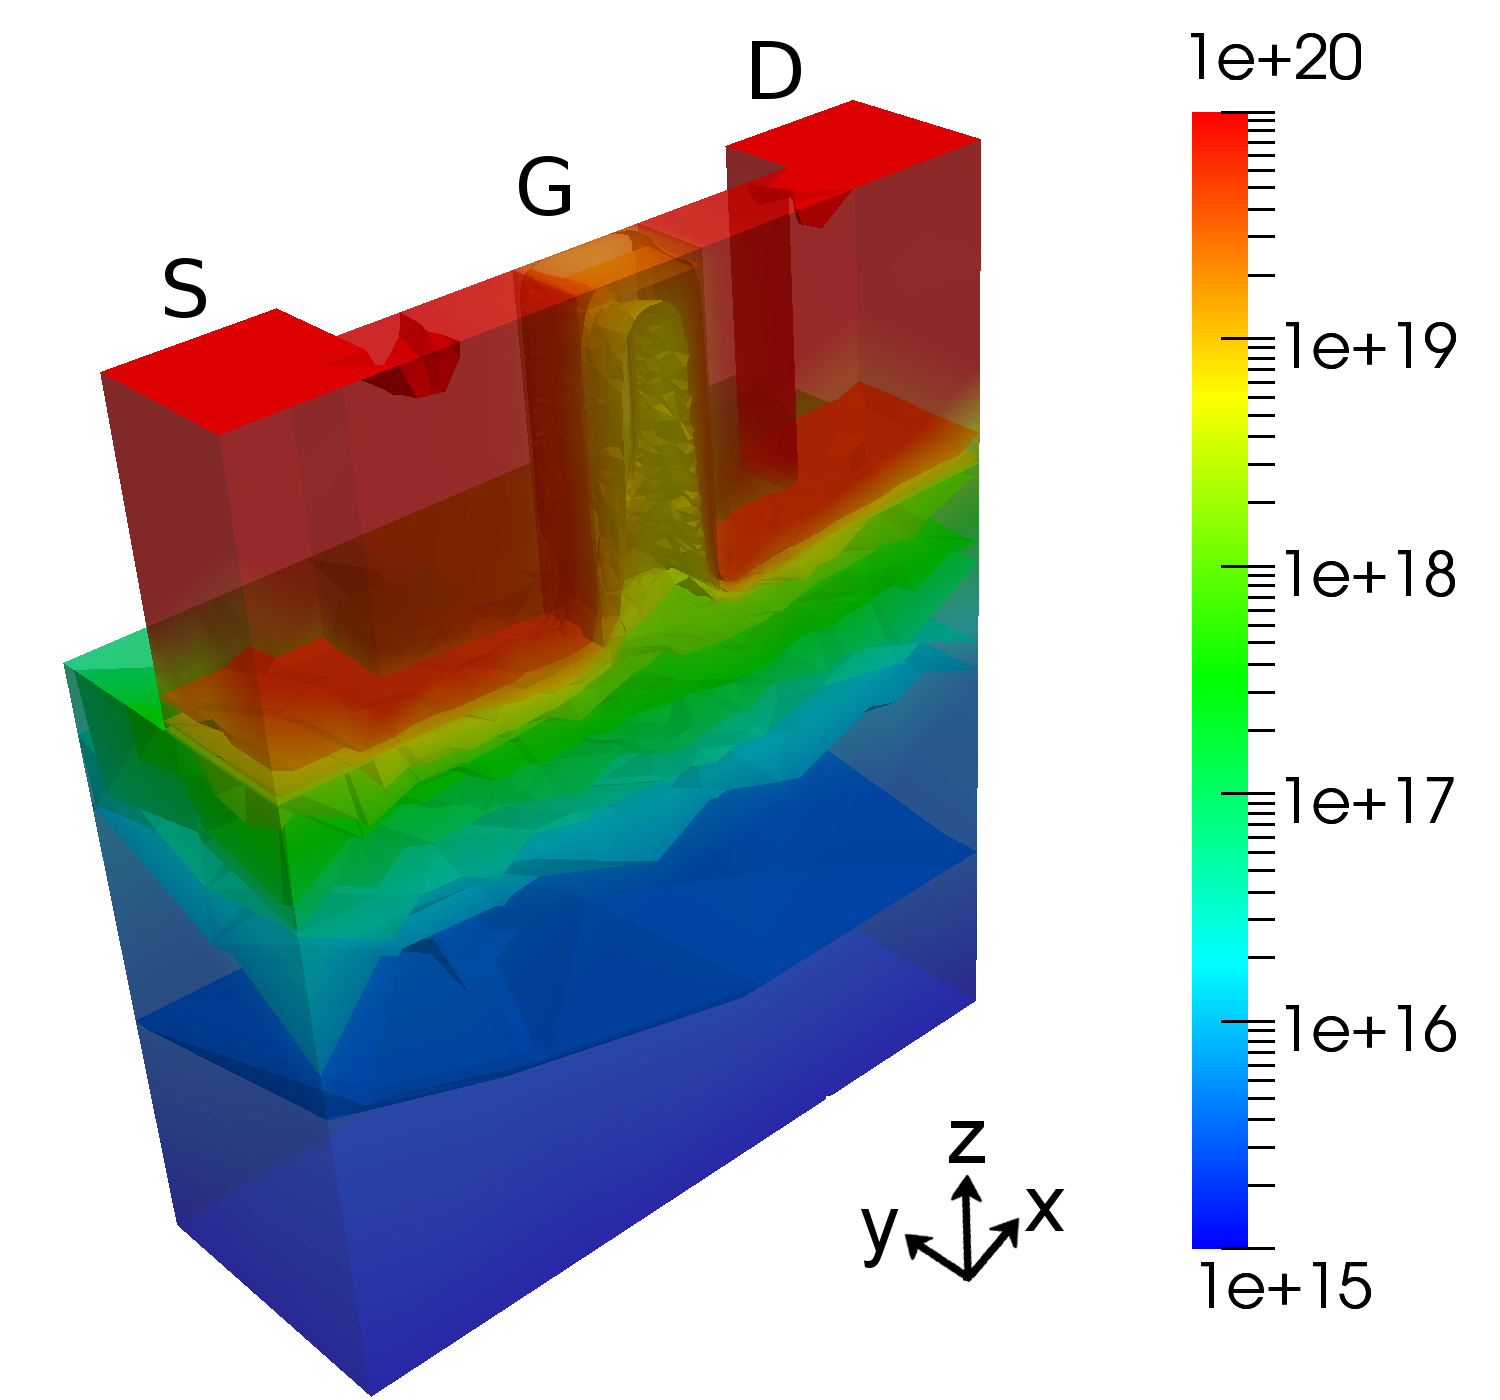
\includegraphics[width=0.6\textwidth]{trigate-n-2}
 \end{center} 
 
\end{frame} 


\begin{frame} {Electron Density in a FinFET} 
  
 \begin{center} 
  Density of electrons at each point $\mathbf x$ \\ 
  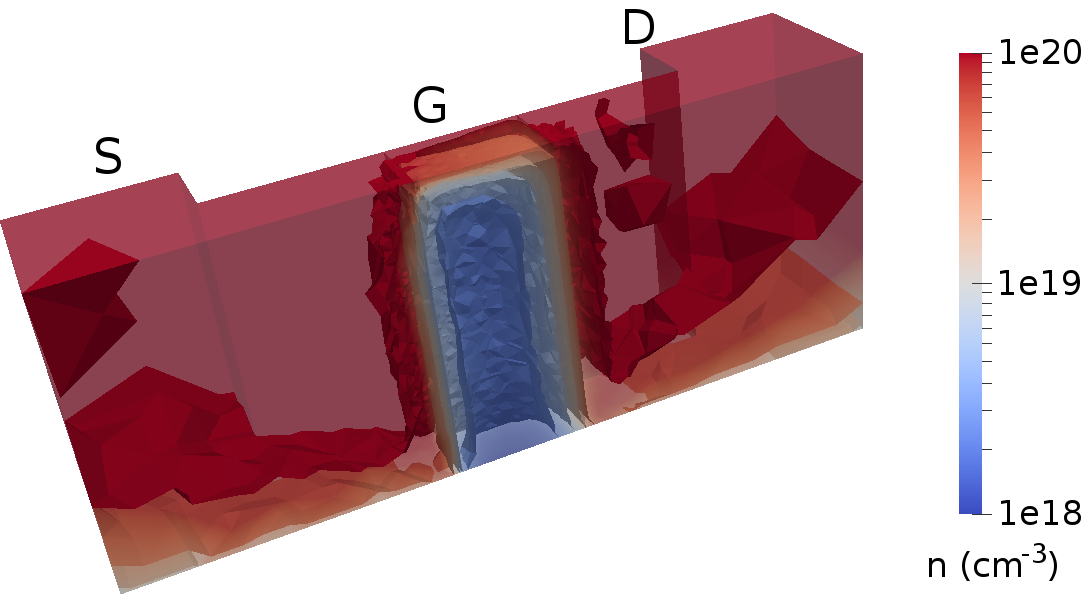
\includegraphics[width=0.632\textwidth]{trigate-electrons-mod}
 \end{center} 
  \vspace*{2.68cm}
 
\end{frame} 
 

\begin{frame} {Electron Energy Distribution?} 
 \begin{center}Distribution of electrons with respect to energy at $\mathbf{x}$? \\ 
  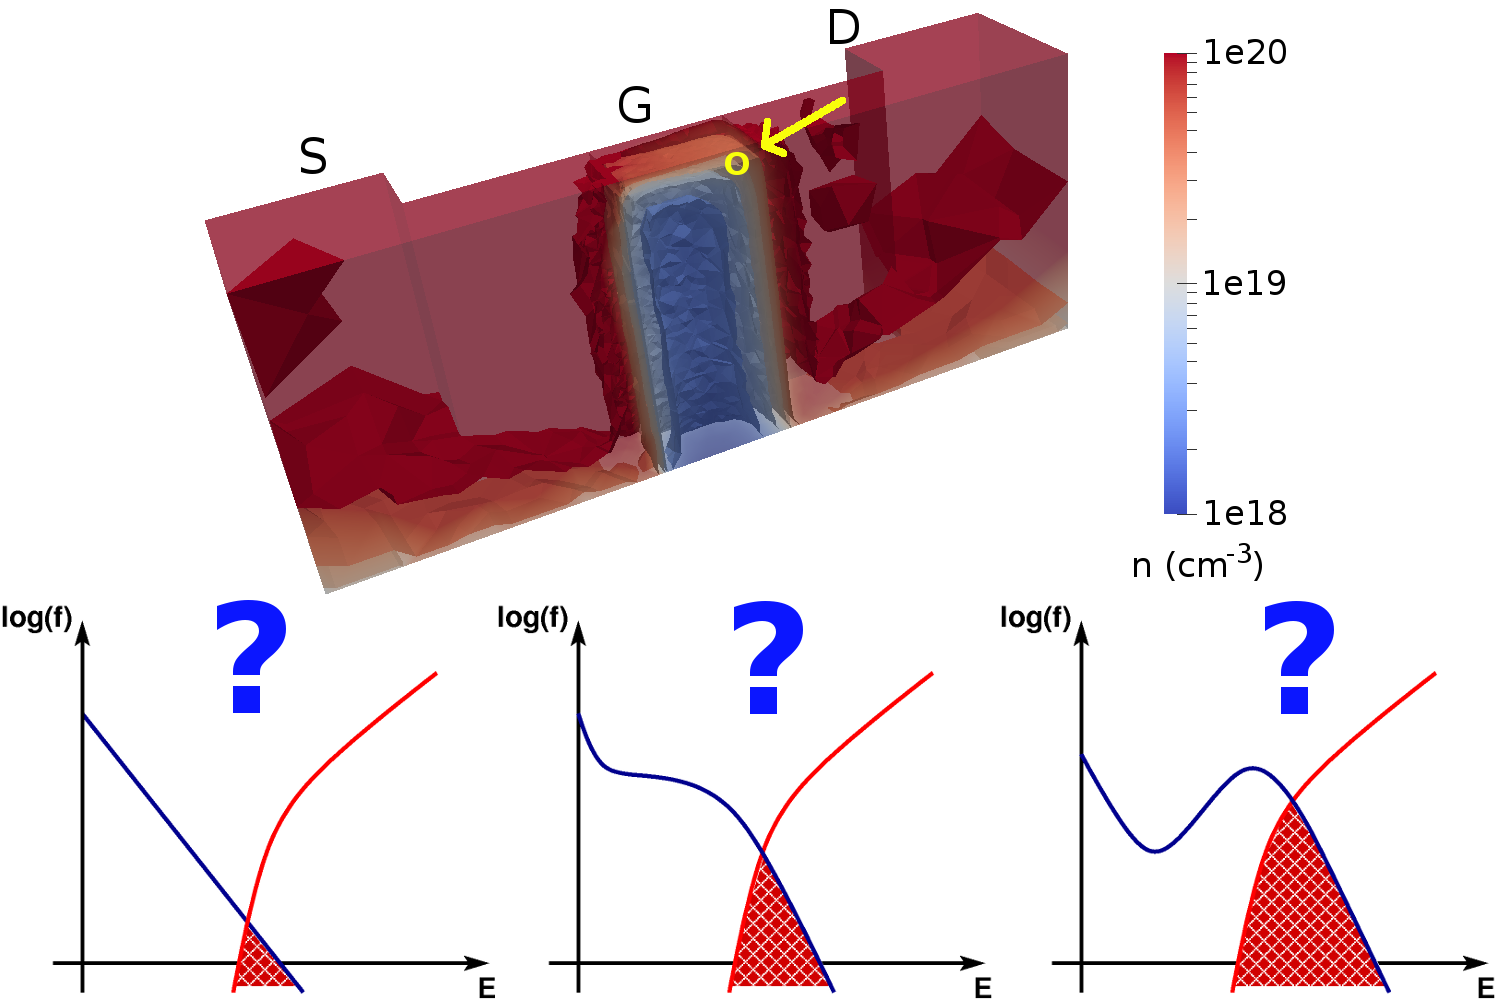
\includegraphics[width=0.87\textwidth]{trigate-electrons-edf-3}
 \end{center} 
\end{frame} 
 

\begin{frame} {Electron Energy Distribution?} 
 
  \begin{block}{Macroscopic Transport Models} 
    \begin{itemize} 
     \item Invalid in deca-nanometer regime 
     \item ``Fitting'' only treats the symptoms, not the cause 
     \item Only averaged quantities of the carrier ensemble modeled 
    \end{itemize} 
  \end{block} 
 
 %\visible<2->{
  \vspace*{0.5cm}
  \begin{block}{Boltzmann Transport Equation (BTE)} 
    \begin{align*} \Large 
      \frac{\partial f}{\partial t} +  \mathbf{v}(\mathbf{k}) \cdot \nabla_{\mathbf{x}} f + \mathbf F(\mathbf x) \cdot \nabla_{\mathbf k} f = Q\{f\}  
    \end{align*} 
  \vspace*{0.1cm}
 
    \begin{itemize} 
      \item Best semi-classical description of carrier transport 
      \item Posed in a seven-dimensional $(\mathbf x, \mathbf k, t)$ space 
      \item Most popular solution method: Monte Carlo 
    \end{itemize} 
  \end{block} 
  \vspace*{0.5cm}
  %}
\end{frame} 
 


\begin{frame} {Electron Energy Distribution?}
 \begin{center}
  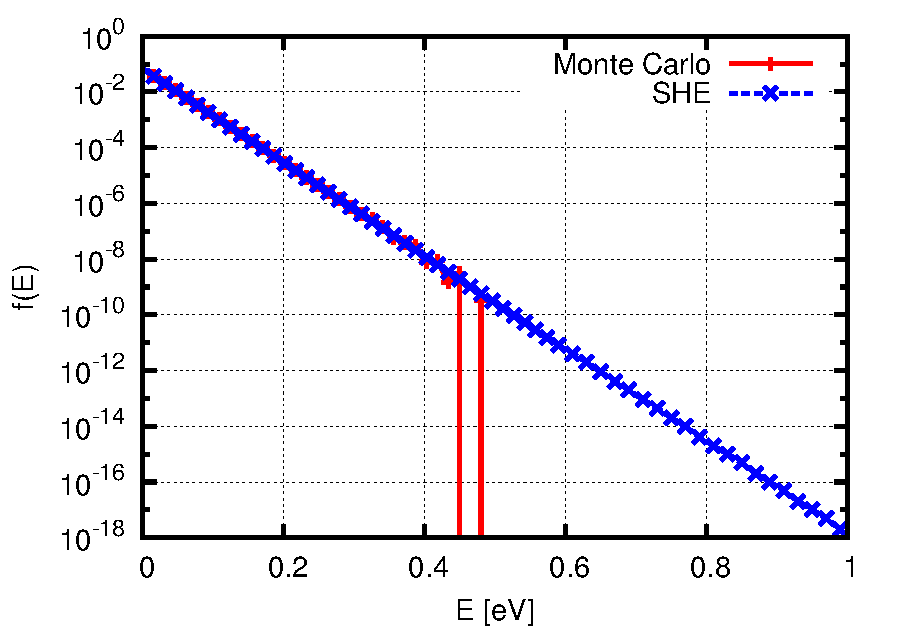
\includegraphics[width=0.95\textwidth]{she-monte-carlo-2}
 \end{center}
\end{frame}
 

\section{Spherical Harmonics Expansion Method}




\begin{frame}{Spherical Harmonics Expansion Method}

 \vspace*{-0.3cm}
  \begin{block}{Spherical Symmetries}
  \begin{itemize}
   \item Maxwell distribution of carriers at equilibrium
   \item Dispersion relation (Herring-Vogt transform, approx.)
  \end{itemize}
  \end{block}

 
     \vspace*{0.62cm}
  \begin{block}{Spherical Harmonics Expansion (SHE)}
     \vspace*{-0.5cm}
      { %\Large
       \begin{align*}
	f(\mathbf x, \mathbf k, t) \simeq \sum_{l = 0}^L \sum_{m=-l}^l f_{l,m}(\mathbf x, E, t) Y_{l,m}(\theta, \varphi)
      \end{align*}}
     \vspace*{-0.5cm}
    \begin{itemize}
     \item New unknowns: $f_{l,m}(\mathbf x, E, t)$
     \item Solution in five-dimensional $(\mathbf x, E, t)$-space
     \item S.-M.~Hong and C.~Jungemann, \textit{J Comput Electron} (2009): \\
           Fifth-order, three-dim.~$(\mathbf x, E)$-space, 26 GB memory, 12 hours
    \end{itemize}
   \end{block}
%     \vspace*{-0.4cm}


\end{frame}



